\chapter{Experiments}
\label{sec:experiments}

Our final dataset for training the triplet loss model consisted of 20000 triplets, gradually accumulated through our labeling application. We employed consistent training configurations (\autoref{sec:training-setups}). The experiments were conducted using two different model architectures : GNN (\autoref{sec:graph-based-models}) and Transformer-based models (\autoref{sec:transformer-based-models}). 

\section{Training setups}
\label{sec:training-setups}

\subsection{Data}

The dataset used for training the models consists of 20000 triplets, each containing three 3D pieces: an anchor, a positive, and a negative model. Input data are meshes stored in stl files.

For the GNN model, vertices of the mesh are represented as nodes in a graph, while edges are defined based on the connectivity of the vertices. When two vertices share a face, an edge is created between them. 
For the transformer model, that take as input a point cloud, we convert the mesh into a point cloud by sampling points uniformly from the surface of the mesh. The number of sampled points is fixed to 10000, following \cite{liuOpenShapeScaling3D2023}.

Initially, the use of Principal Component Analysis (PCA) for training or inference, as done in \cite{popRotationInvariantGraph2023}, was considered but ultimately discarded. The idea of PCA is appealing because it allows working within a canonical reference frame. However, to ensure the model is as general as possible, data augmentation techniques were favored over PCA. One of the issues with PCA is demonstrated in \autoref{fig:pca_problem}. Additionally, we prefer to let the model architecture handle these aspects directly.

\begin{figure}[]
    \centering
    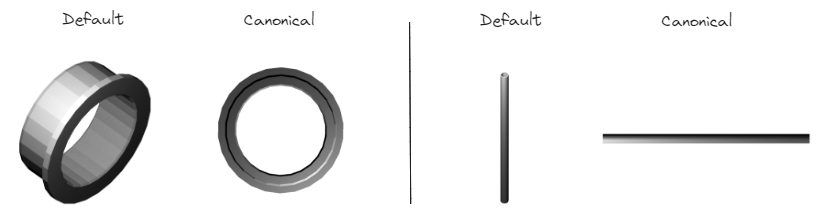
\includegraphics[width=\columnwidth]{images/pca_problem.png}
    \caption{Illustration of the issue using PCA as a preprocessing step. Both pieces are tubular structures, shown in their default orientation and in the canonical reference frame. While the piece on the left aligns its first principal axis with the tube's axis, the piece on the right does not. This inconsistency can result in misalignment during training, particularly since the behavior varies depending on the specific piece.}
    \label{fig:pca_problem}
\end{figure}

Data augmentation was performed to enhance the model's robustness, especially considering rotations. Other augmentation techniques, such as symmetry and noise addition, were also explored but ultimately discarded. The following two techniques were retained:
\begin{enumerate}
    \item \textbf{Normalization to unit sphere}: We standardize all the pieces to fit within a unit sphere. This enhances the model's ability to capture geometric features rather than scale. The length of the piece has been integrated into the architecture of the GNN model.
    \item \textbf{Random rotations}: Each piece is randomly rotated around the three axes. This is crucial for ensuring that the model learns to recognize pieces regardless of their orientation. A special focus was placed on rotation invariance, as explained hereafter.
\end{enumerate}

Rotation invariance is a critical aspect of our model, as it allows the model to recognize pieces regardless of their orientation. This is particularly important in our context since 3D model designers often work with similar pieces saved in different orientations. To achieve this, 3 metrics were defined to evaluate the model's performance in terms of rotation invariance:
\begin{itemize}
    \item \textbf{Mean distance to rotated distribution}: This metric calculates the average distance between the model's prediction of a piece and the predictions of its $n$ rotated versions. 
    \item \textbf{Median distance to rotated distribution}: Similar to the mean distance, this metric computes the median distance between the model's prediction and the predictions of the $n$ rotated versions.
    \item \textbf{Rotation matching accuracy}: The two previous metrics are absolute. To provide a more relative measure, we also compute a rotation matching accuracy. If we fix a value of $n$, we can compute the proportion of nearest neighbors in the whole dataset that are also among the $n$ rotated versions of the piece. $n$ is set to 10 in our experiments, as for the two previous metrics.
\end{itemize}

Initially, data augmentation was performed offline. This means that for each triplet, each piece was augmented by applying random rotations before the training process. We choose 10 rotations per piece, as it yields the best results as shown in \autoref{fig:rotated_study}. Results are shown with our starting GNN EdgeConv model.
\begin{figure}[]
    \begin{subfigure}[h]{0.5\linewidth}
        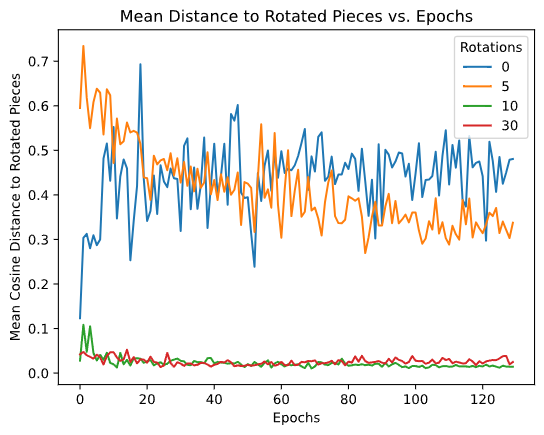
\includegraphics[width=\columnwidth]{images/mean_rotated_study.png}
        \caption{Mean distance to rotated distribution.}
        \label{fig:mean_rotated_study}
    \end{subfigure}
    \hfill
    \begin{subfigure}[h]{0.5\linewidth}
        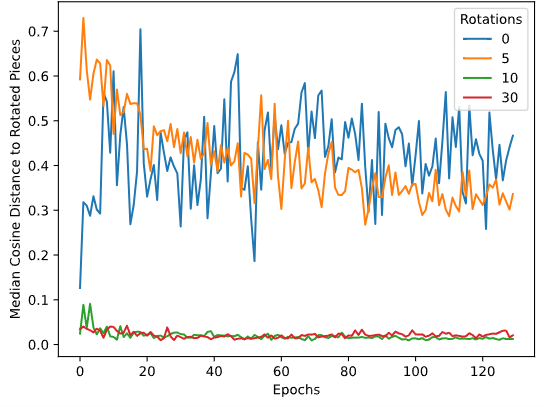
\includegraphics[width=\columnwidth]{images/median_rotated_study.png}
        \caption{Median distance to rotated distribution.}
        \label{fig:median_rotated_study}
    \end{subfigure}
    \caption{Influence of the number of rotations on the rotations metrics.}
    \label{fig:rotated_study}
\end{figure}

We also experienced online data augmentation, where random rotations are applied on-the-fly during training. Indeed, there is no clear recipe for the best approach \cite{OfflineDataAugmentation} and we wanted to explore both options. The results of both approaches are compared in \autoref{fig:augmented_data_comparison}. The offline augmentation approach yielded better results.
\begin{figure}[]
    \begin{subfigure}[h]{0.5\linewidth}
        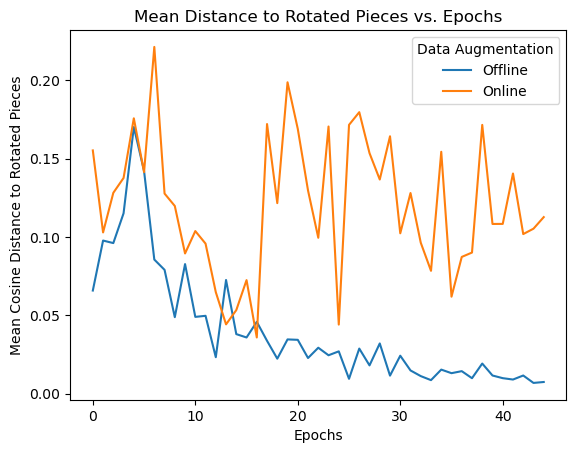
\includegraphics[width=\columnwidth]{images/mean_rotated_data_augmentation_type.png}
        \caption{Mean distance to rotated distribution.}
        \label{fig:mean_rotated_data_augmentation_type}
    \end{subfigure}
    \hfill
    \begin{subfigure}[h]{0.5\linewidth}
        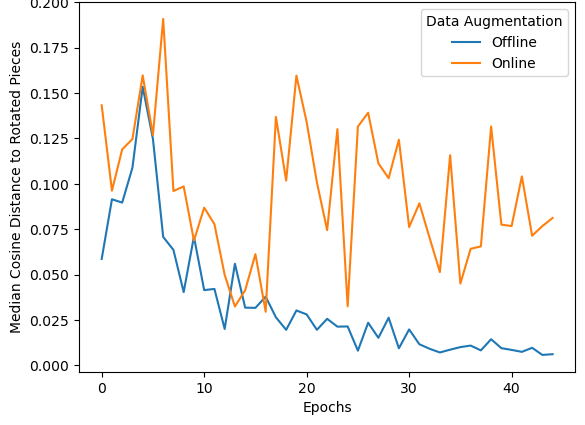
\includegraphics[width=\columnwidth]{images/median_rotated_data_augmentation_type.png}
        \caption{Median distance to rotated distribution.}
        \label{fig:median_rotated_data_augmentation_type}
    \end{subfigure}
    \caption{Influence of the type of data augmentation on the rotations metrics.}
    \label{fig:augmented_data_comparison}
\end{figure}

\subsection{Triplets metrics}

As is described in TODO, training a triplet loss model is notoriously difficult. To better monitor the training process, several metrics were defined:
\begin{itemize}
    \item \textbf{Train easy triplets proportion}: This metric computes the proportion of easy triplets in the training set. An easy triplet results in a loss of 0.
    \item \textbf{Test easy triplets proportion}: This metric computes the proportion of easy triplets in the test set. 
    \item \textbf{Training triplets order}: This metrics computes the proportion of triplets that are 'correctly' ordered. A triplet is correctly ordered if the distance between the anchor and positive is less than the distance between the anchor and negative. This is the same as an easy triplet proportion for a triplet loss with margin 0.
    \item \textbf{Test triplets order}: This metrics computes the proportion of triplets that are 'correctly' ordered in the test set.
\end{itemize}


Proportions of the training data were incorporated to analyze the model's behavior when converging to a loss of 0. The order of triplets was included to both assess the impact of the margin on triplet loss and to align with the fact that this order ultimately matters, as it's the one used by app users for labeling.

In addition to the rotation metrics, we also computed the accuracy of the model on the small labeled dataset by evaluating the proportion of pieces which nearest neighbor shares the same label. This metric is referred to as the \textbf{test accuracy}.

\section{Graph-based models}
\label{sec:graph-based-models}
\begin{figure}[]
    \centering
    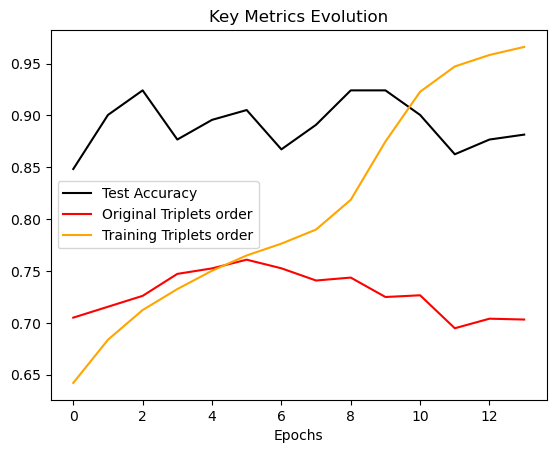
\includegraphics[width=0.5\columnwidth]{images/key_metrics_evolution_gnn.png}
    \caption{GNN model key metrics accuracies.}
    \label{fig:key_metrics_evolution_gnn}
\end{figure}


\section{Transformer-based models}
\label{sec:transformer-based-models}

\begin{figure}[]
    \centering
    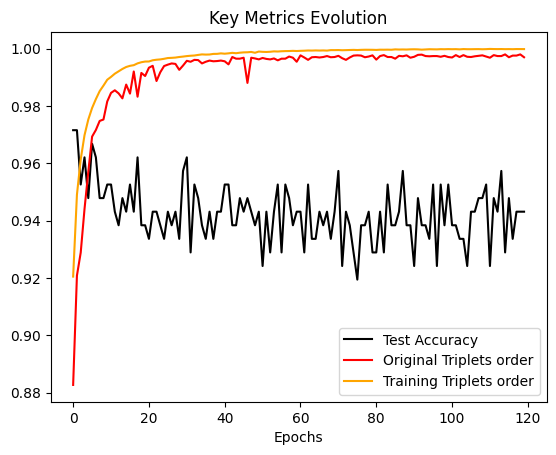
\includegraphics[width=0.5\columnwidth]{images/key_metrics_evolution_openshape.png}
    \caption{Fine-tuned model key metrics accuracies.}
    \label{fig:key_metrics_evolution_openshape}
\end{figure}

\begin{figure}[]
    \begin{subfigure}[h]{0.5\linewidth}
        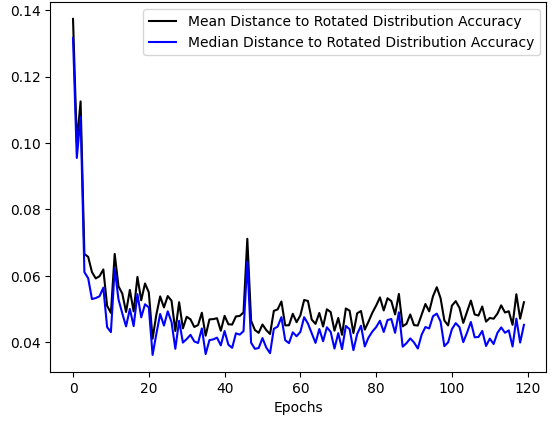
\includegraphics[width=\columnwidth]{images/rotation_metrics_evolution_openshape.png}
        \caption{Distances to rotated pieces accuracies.}
    \end{subfigure}
    \hfill
    \begin{subfigure}[h]{0.5\linewidth}
        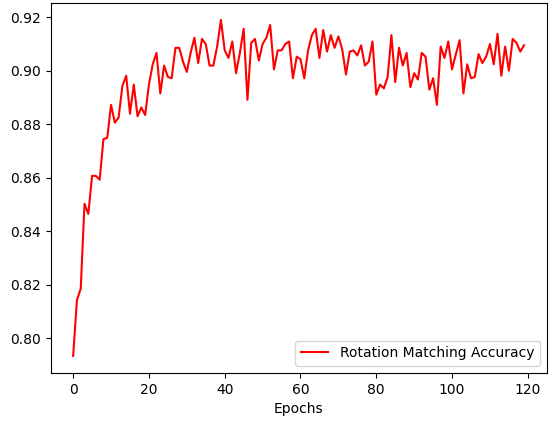
\includegraphics[width=\columnwidth]{images/rotation_accuracy_evolution_openshape.png}
        \caption{Rotation matching accuracy.}
    \end{subfigure}
    \caption{Fine-tuned model rotation accuracies.}
\end{figure}

%%% Local Variables: 
%%% mode: latex
%%% TeX-master: "isae-report-template"
%%% End: 